\section{Modellazione del problema}

La simulazione del problema prevede la creazione di una popolazione iniziale
di cellule basata su un istogramma fornito in input denominato $H(0)$
contenente coppie di valori ($\varphi_{i}, \psi_{i}$),
con $\varphi_{i} \in \R, \psi_{i} \in \N$ indicanti rispettivamente il
valore di fluorescenza rilevato dalle misurazioni in laboratorio e
la frequenza con il quale esso si presenta.
La popolazione iniziale di cellule è rappresentabile tramite un array di
lunghezza pari a $$L = \sum_{i=1}^{|\varphi|} \psi_{i}$$

\begin{figure}[H]
\centering
\begin{tikzpicture}
    \pgftransparencygroup
    \nodes{$\varphi_{0}$,$\varphi_{0}$}
    \endpgftransparencygroup
    \pgftransparencygroup
    \nodes{$\varphi_{1}$,$\varphi_{1}$,$\varphi_{1}$}
    \endpgftransparencygroup
    \pgftransparencygroup
    \hiddennodes{.,.,.}
    \endpgftransparencygroup
    \pgftransparencygroup
    \nodes{$\varphi_{n}$,$\varphi_{n}$}
    \endpgftransparencygroup
    \pgftransparencygroup
    \brckt{1}{2}{0}{$\psi_{0}$}
    \endpgftransparencygroup
    \pgftransparencygroup
    \brckt{3}{5}{0}{$\psi_{1}$}
    \endpgftransparencygroup
    \pgftransparencygroup
    \brckt{9}{10}{0}{$\psi_{n}$}
    \endpgftransparencygroup
    \pgftransparencygroup
    \brckt{1}{10}{2}{$L$}
    \endpgftransparencygroup
\end{tikzpicture}
\caption{Rappresentazione di una popolazione di cellule mediante array}
\end{figure}

Ad ogni fenomeno di divisione cellulare corrisponde
la creazione di due nuove cellule aventi valore di fluorescenza dimezzato
rispetto alla cellula originaria.
Questo comportamento è modellabile tramite un albero binario bilanciato

\begin{figure}[H]
\centering
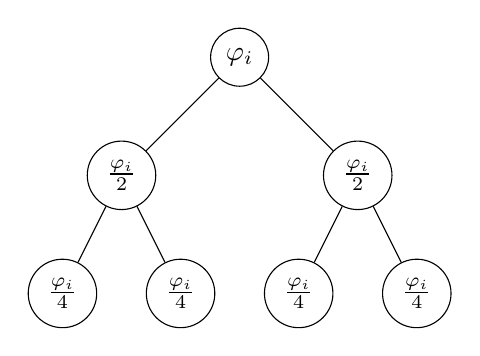
\begin{tikzpicture}[level/.style={sibling distance=30mm/#1}]
    \node [circle, draw] (a) {$\varphi_{i}$}
        child {
            node [circle,draw] (b) {$\frac{\varphi_{i}}{2}$}
                child {
                    node [circle,draw] (d) {$\frac{\varphi_{i}}{4}$}
                }
                child {
                    node [circle,draw] (e) {$\frac{\varphi_{i}}{4}$}
                }
        }
        child {
            node [circle,draw] (c) {$\frac{\varphi_{i}}{2}$}
                child {
                    node [circle,draw] (f) {$\frac{\varphi_{i}}{4}$}
                }
                child {
                    node [circle,draw] (g) {$\frac{\varphi_{i}}{4}$}
                }
        };
\end{tikzpicture}
\caption{Rappresentazione di divisione cellulare tramite albero binario
    bilanciato}
\end{figure}

La popolazione iniziale di cellule dunque dà vita ad insieme di $L$ alberi di
divisione. Il primo livello di questo insieme corrisponde alla popolazione
iniziale di cellule, di conseguenza ogni livello successivo rappresenterà
un nuovo stadio di proliferazione cellulare avente popolazione con numerosità
uguale a $L * 2^{i}$ con $i$ uguale al livello considerato.
Quindi se il primo livello dell'albero corrisponde all'array della popolazione
iniziale, allora anche ad ogni livello successivo corrisponde un array i quali
elementi sono le nuove cellule ottenute dalla divisione cellulare del livello
immediatamente precedente.
In definitiva la totalità dei fenomeni di proliferazione è descritta da un
insieme di array, dove ognuno racchiude tutte e sole le cellule
corrispondenti ad uno specifico livello degli alberi di proliferazione generati
a partire dalla popolazione iniziale.
